\documentclass{standalone}
\usepackage{tikz}
\begin{document}
 % Make the whole figure wider (x-direction).
 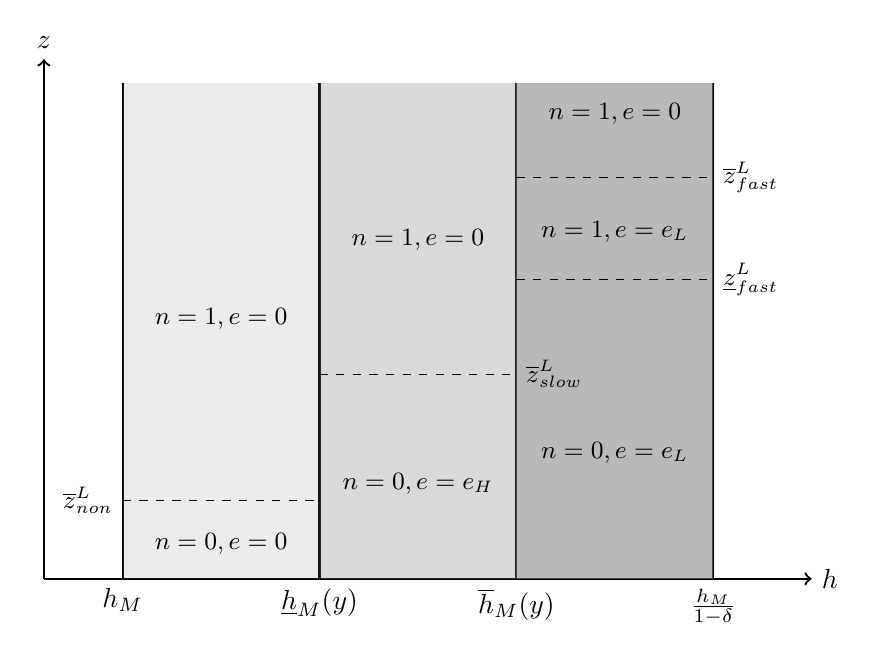
\begin{tikzpicture}[xscale=1.25]

% Decision rule conditional on a given y:
% x-axis: h in [h_M, h_M/(1-delta))
% y-axis: z

% Axes
\draw[thick,->] (-0.8,0) -- (7,0) node[right] {$h$};
\draw[thick,->] (-0.8,0) -- (-0.8,6.6) node[above] {$z$};

% h-range boundaries
\draw[thick] (0,0) -- (0,6.3);
\node[below] at (0,0) {$h_M$};
\draw[thick] (6,0) -- (6,6.3);
\node[below] at (6,0) {$\frac{h_M}{1-\delta}$};


% Learner-type cutoffs in h conditional on y (schematic placement)
\draw[thick] (2,0) -- (2,6.3);
\draw[thick] (4,0) -- (4,6.3);
\node[below] at (2,0) {$\underline{h}_M(y)$};
\node[below] at (4,0) {$\overline{h}_M(y)$};

% Shade learner-type regions (conditional on y)
\fill[gray, opacity=0.15] (0,0) rectangle (2,6.3); % non-learners
\fill[gray, opacity=0.30] (2,0) rectangle (4,6.3); % slow learners
\fill[gray, opacity=0.55] (4,0) rectangle (6,6.3); % fast learners

% z cutoffs (schematic heights)
\def\zNon{1.0}
\def\zSlow{2.6}
\def\zFastL{3.8}
\def\zFastU{5.1}

% Non-learner cutoff
\draw[dashed] (0,\zNon) -- (2,\zNon);
\node[left] at (0,\zNon) {\small $\overline{z}^L_{non}$};

% Slow-learner cutoff
\draw[dashed] (2,\zSlow) -- (4,\zSlow);
\node[right] at (4,\zSlow) {\small $\overline{z}^L_{slow}$};

% Fast-learner cutoffs
\draw[dashed] (4,\zFastL) -- (6,\zFastL);
\draw[dashed] (4,\zFastU) -- (6,\zFastU);
\node[right] at (6,\zFastL) {\small $\underline{z}^L_{fast}$};
\node[right] at (6,\zFastU) {\small $\overline{z}^L_{fast}$};

% Decision labels inside regions
% Non-learners
\node at (1,0.45) {\small $n=0,e=0$};
\node at (1,3.3) {\small $n=1,e=0$};

% Slow learners
\node at (3,1.2) {\small $n=0,e=e_H$};
\node at (3,4.3) {\small $n=1,e=0$};

% Fast learners
\node at (5,1.6) {\small $n=0,e=e_L$};
\node at (5,4.4) {\small $n=1,e=e_L$};
\node at (5,5.9) {\small $n=1,e=0$};

\end{tikzpicture}

\end{document}
